% Generated from reviewed lane; compile via book/textbook.tex.
\clearpage

原书 PDF 页 58；印刷页码 45。

\href{source-images/pdf-058.jpeg}{查看原页}

\section{第 3 章 函数逼近与计算}\label{ch03a-ux7b2c-3-ux7ae0-ux51fdux6570ux903cux8fd1ux4e0eux8ba1ux7b97}

\subsection{3.1 引言与预备知识}\label{ch03a-ux5f15ux8a00ux4e0eux9884ux5907ux77e5ux8bc6}

\subsubsection{3.1.1 问题的提出}\label{ch03a-ux95eeux9898ux7684ux63d0ux51fa}

在数值计算中经常遇到求函数值的问题. 用手工计算时常常通过函数表求得; 用计算机计算时, 若把函数表存入内存进行查表, 则占用单元太多, 不如直接用公式计算方便. 因此, 我们希望求出便于计算且计算量省的公式近似已知函数 \(f(x)\). 例如, Taylor 展开式的部分和

\[
P_n(x) = f(x_0) + \frac{f'(x_0)}{1!}(x-x_0) + \cdots + \frac{f^{(n)}(x_0)}{n!}(x-x_0)^n \tag{3.1.1}
\]

就是 \(f(x)\)的一种近似公式. 用它求 \(x_0\) 附近的函数值 \(f(x)\) 误差较小, 当 \(|x-x_0|\) 较大时误差就很大. 例如 \(f(x)=e^x\) 在 \([-1,1]\) 上用

\[
P_4(x) = 1+x+\frac{1}{2}x^2+\frac{1}{6}x^3+\frac{1}{24}x^4
\]

近似 \(e^x\), 其误差

\[
R_4(x)=e^x-P_4(x)=\frac{1}{120}x^5e^\epsilon, \quad \epsilon \in(-1,1),
\]

于是

\[
|R_4(x)| \leqslant \frac{e}{120}|x^5|, \quad \max_{-1 \leqslant x \leqslant 1}|R_4(x)| \leqslant \frac{e}{120} \approx 0.0226.
\]

误差分布如图3.1所示, 它在整个区间上误差较大. 若在计算机上用这种方法计算 \(e^x\), 如精度要求较高, 则需取很多项, 这样既费时又多占存储单元, 因此, 要求在给定精度下求计算次数最少的近似公式, 这就是函数逼近与计算要解决的问题. 这问题可叙述为: ``对于函数类 \(A\) 中给定的函数 \(f(x)\), 要求在另一类较简单的便于计算的函数类 \(B\) 中, 求函数 \(P(x) \in B \subseteq A\), 使 \(P(x)\) 与 \(f(x)\) 之差在某种度量意义下最小.'' 函数类 \(A\) 通常是区间 \([a,b]\) 上的连续函数, 记作 \(C[a,b]\); 函数类 \(B\) 通常是代数多项式、分式有理函数或三角多项式. 而度量标准最常用的有两种,一种是

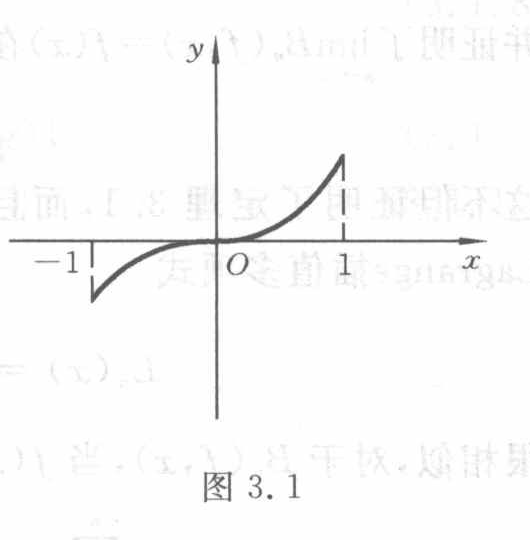
\includegraphics[width=0.85\linewidth,height=\textheight,keepaspectratio,alt={图 3.1 原图裁切}]{verified/assets/ch03a/fig-3-1.png}

图 3.1（原图）。图中为上文误差分布曲线，横轴 \(x\)、纵轴 \(y\)；标签为 \(-1\)、\(1\)、\(O\)。曲线在负半轴下方、正半轴上方，通过原点；在 \(x=-1\) 和 \(x=1\) 处有竖向辅助线。

\clearpage

原书 PDF 页 59；印刷页码 46。

\href{source-images/pdf-059.jpeg}{查看原页}

\[
\| f(x) - P(x) \|_{\infty} = \max_{a \leqslant x \leqslant b} |f(x) - P(x)|, \tag{3.1.2}
\]

在这种度量意义下的函数逼近称为一致逼近或均匀逼近；另一种度量标准是 \[
\| f(x) - P(x) \|_{2} = \sqrt{\int_{a}^{b} [f(x) - P(x)]^{2} \mathrm{d}x}, \tag{3.1.3}
\]

用这种度量的函数逼近称为均方逼近或平方逼近. 这里, 符号 \(\| \cdot \|_{\infty}\) 及 \(\| \cdot \|_{2}\) 是范数. 本章主要研究在这两种度量标准下用代数多项式 \(P_{n}(x)\) 逼近 \(f(x) \in C[a,b]\), 也就是用最佳一致逼近多项式与最佳平方逼近多项式逼近 \(f(x) \in C[a,b]\).

\subsubsection{3.1.2 Weierstrass 定理}\label{ch03a-weierstrass-ux5b9aux7406}

用插值法或 Taylor 展开求 \(f(x) \in C[a,b]\) 的逼近多项式, 在某些点上可能没有误差, 但在整个区间 \([a,b]\) 上误差可能很大, 2.7 节给出的 Runge 现象就说明了这一点. 因此, 用 \(P_{n}(x)\) 一致逼近 \(f(x)\), 首先要解决存在性问题, 即对于 \([a,b]\) 上的连续函数 \(f(x)\), 是否存在多项式 \(P_{n}(x)\) 一致收敛于 \(f(x)\)? Weierstrass 给出了下面定理.

定理 3.1 设 \(f(x) \in C[a,b]\), 则对于任何 \(\varepsilon > 0\), 总存在一个代数多项式 \(P(x)\), 使 \[
\| f(x) - P(x) \|_{\infty} < \varepsilon
\] 在 \([a,b]\) 上一致成立.

这定理已在``数学分析''中证明过. 这里需要说明的是在许多证明方法中, Bernstein 在 1912 年给出的证明是一种构造性证明. 他根据函数整体逼近的特性造出 Bernstein 多项式 \[
\begin{cases} B_{n}(f,x) = \sum_{k=0}^{n} f\left(\frac{k}{n}\right) P_{k}(x), \\ P_{k}(x) = \binom{n}{k} x^{k}(1-x)^{n-k}, \end{cases} \tag{3.1.4}
\]

并证明了 \(\lim_{n \to \infty} B_{n}(f,x) = f(x)\) 在 \([0,1]\) 上一致成立; 若 \(f(x)\) 在 \([0,1]\) 上 \(m\) 阶导数连续, 则 \[
\lim_{n \to \infty} B_{n}^{(m)}(f,x) = f^{(m)}(x).
\] 这不但证明了定理 3.1, 而且由式 (3.1.4)给出了 \(f(x)\) 的一个逼近多项式. 它与 Lagrange 插值多项式 \[
L_{n}(x) = \sum_{k=0}^{n} f\left(x_{k}\right) l_{k}(x), \quad \sum_{k=0}^{n} l_{k}(x_{k}) = 1
\] 很相似, 对于 \(B_{n}(f,x)\), 当 \(f(x)=1\) 时也有关系式 \[
\sum_{k=0}^{n} P_{k}(x) = \sum_{k=0}^{n} \binom{n}{k} x^{k}(1-x)^{n-k} = 1. \tag{3.1.5}
\]

这只要从恒等式

\begin{quote}
校注（agent 补充，原书疑误）：原页 Lagrange 插值式后的求和明确印为 \(\sum_{k=0}^{n}l_k(x_k)=1\)，此处按原文保留。由基函数性质 \(l_k(x_k)=1\)，左端应为 \(n+1\)；通常的恒等式应为 \(\sum_{k=0}^{n}l_k(x)=1\)。这不是 OCR 误识。
\end{quote}

\clearpage

原书 PDF 页 60；印刷页码 47。

\href{source-images/pdf-060.jpeg}{查看原页}

\[
(x+y)^n = \sum_{k=0}^{n} \binom{n}{k} x^k y^{n-k} \tag{3.1.6}
\] 中令 \(y=1-x\) 就可得到. 但这里当 \(x \in [0,1]\) 时还有 \(P_k(x) \geqslant 0\), 于是 \[
\sum_{k=0}^{n} |P_k(x)| = \sum_{k=0}^{n} P_k(x) = 1
\] 是有界的, 因而只要 \(|f(x)| \leqslant \delta\) 对于任意 \(x \in [0,1]\) 成立, 则 \[
|B_n(f,x)| \leqslant \max_{0 \leqslant x \leqslant 1} |f(x)| \sum_{k=0}^{n} |P_k(x)| \leqslant \delta
\] 有界, 故 \(B_n(f,x)\) 是稳定的. 至于 Lagrange 插值多项式 \(L_n(x)\), 由于 \(\sum_{k=0}^{n} |l_k(x)|\) 无界, 因而不能保证高阶插值的稳定性与收敛性. 相比之下, 多项式 \(B_n(f,x)\) 有良好的逼近性质, 但它收敛太慢, 比三次样条逼近效果差得多, 实际中很少使用.

\subsubsection{\texorpdfstring{3.1.3 连续函数空间 \(C[a,b]\)}{3.1.3 连续函数空间 C{[}a,b{]}}}\label{ch03a-ux8fdeux7eedux51fdux6570ux7a7aux95f4-cab}

区间 \([a,b]\) 上的所有实连续函数组成一个空间, 记作 \(C[a,b]\). \(f \in C[a,b]\) 的范数定义为 \[
\|f\|_\infty = \max_{a \leqslant x \leqslant b} |f(x)| ,
\] \(\|\cdot\|_\infty\) 称为 \(\infty\)-范数, 它满足范数 \(\|\cdot\|\) 的三个性质: (1) \(\|f\| \geqslant 0\), 当且仅当 \(f \equiv 0\) 时才有 \(\|f\| = 0\); (2) \(\|af\| = |a| \|f\|\) 对于任意 \(f \in C[a,b]\) 成立, \(a\) 为任意实数; (3) 对于任意 \(f,g \in C[a,b]\), 有 \[
\|f+g\| \leqslant \|f\| + \|g\| \tag{3.1.7}
\] 式(3.1.7)称为三角不等式. 空间 \(C[a,b]\) 可与向量空间类比, 函数 \(f \in C[a,b]\) 可看成向量. 与向量空间类似, 当 \(f,g \in C[a,b]\) 时, 定义 \(f\) 与 \(g\) 的距离为 \[
D(f,g) = \|f-g\|_\infty \tag{3.1.8}
\] 由式(3.1.7)可得到 \[
D(f,g) \leqslant D(f,h) + D(h,g) \tag{3.1.9}
\] \[
\bigl|\|f\|_\infty - \|g\|_\infty\bigr| \leqslant \|f-g\|_\infty \tag{3.1.10}
\]

\subsection{3.2 最佳一致逼近多项式}\label{ch03a-ux6700ux4f73ux4e00ux81f4ux903cux8fd1ux591aux9879ux5f0f}

\subsubsection{3.2.1 最佳一致逼近多项式的存在性}\label{ch03a-ux6700ux4f73ux4e00ux81f4ux903cux8fd1ux591aux9879ux5f0fux7684ux5b58ux5728ux6027}

Chebyshev 从另一观点研究一致逼近问题. 他不让多项式次数 \(n\) 趋于无穷,

\clearpage

原书 PDF 页 61；印刷页码 48。

\href{source-images/pdf-061.jpeg}{查看原页}

而是固定 \(n\), 记次数不大于 \(n\) 的多项式集合为 \(H_n\), 显然 \(H_n \subseteq C[a,b]\). 又记 \(H_n = \text{span}\{1,x,\cdots,x^n\}\), 其中 \(1,x,\cdots,x^n\) 是 \([a,b]\) 上一组线性无关的函数组, 是 \(H_n\) 中的一组基. \(H_n\) 中的元素 \(P_n(x)\) 可表示为 \[
P_n(x) = a_0 + a_1x + \cdots + a_nx^n,
\] 其中 \(a_0,a_1,\cdots,a_n\) 为任意实数. 要在 \(H_n\) 中求 \(P_n^*(x)\) 逼近 \(f(x) \in C[a,b]\), 使其误差 \[
\max_{a \leqslant x \leqslant b} |f(x) - P_n^*(x)| = \min_{P_n \in H_n} \max_{a \leqslant x \leqslant b} |f(x) - P_n(x)|,
\] 这就是通常所谓最佳一致逼近或 Chebyshev 逼近问题. 为了说明这一概念, 先给出以下定义.

定义 3.1 \(P_n(x) \in H_n, f(x) \in C[a,b]\), 称 \[
\Delta(f,P_n) = \|f - P_n\|_\infty = \max_{a \leqslant x \leqslant b} |f(x) - P_n(x)| \tag{3.2.1}
\] 为 \(f(x)\) 与 \(P_n(x)\) 在 \([a,b]\) 上的偏差.

显然, \(\Delta(f,P_n) \geqslant 0, \Delta(f,P_n)\) 的全体组成一个集合, 记作 \(\{\Delta(f,P_n)\}\), 它有下界 0. 若记集合的下确界为 \[
E_n = \inf_{P_n \in H_n} \{\Delta(f,P_n)\} = \inf_{P_n \in H_n} \max_{a \leqslant x \leqslant b} |f(x) - P_n(x)| \tag{3.2.2}
\] 则称 \(E_n\) 为 \(f(x)\) 在 \([a,b]\) 上的最小偏差.

定义 3.2 假定 \(f(x) \in C[a,b]\), 若存在 \[
P_n^*(x) \in H_n, \Delta(f,P_n^*) = E_n \tag{3.2.3}
\] 则称 \(P_n^*(x)\) 是 \(f(x)\) 在 \([a,b]\) 上的最佳一致逼近多项式或最小偏差逼近多项式, 简称最佳逼近多项式.

注意, 定义并未说明最佳逼近多项式是否存在, 但可证明下面的存在定理.

定理 3.2 若 \(f(x) \in C[a,b]\), 则总存在 \(P_n^*(x) \in H_n\), 使 \[
\|f(x) - P_n^*(x)\|_\infty = E_n.
\] 证明过程见文献{[}4{]}, 此处从略.

\subsubsection{3.2.2 Chebyshev 定理}\label{ch03a-chebyshev-ux5b9aux7406}

这一节要研究最佳逼近多项式的特性, 为此先引进偏差点定义.

定义 3.3 设 \(f(x) \in C[a,b], P(x) \in H_n\), 若在 \(x = x_0\) 上有 \[
|P(x_0) - f(x_0)| = \max_{a \leqslant x \leqslant b}|P(x) - f(x)| = \mu,
\] 则称 \(x_0\) 是 \(P(x)\) 的偏差点.

若 \(P(x_0) - f(x_0) = \mu\), 则称 \(x_0\) 为``正''偏差点.

若 \(P(x_0) - f(x_0) = -\mu\), 则称 \(x_0\) 为``负''偏差点.

由于函数 \(P(x) - f(x)\) 在 \([a,b]\) 上连续, 因此, 至少存在一个点 \(x_0 \in [a,b]\), 使得 \[
|P(x_0) - f(x_0)| = \mu,
\] 也就是说, \(P(x)\) 的偏差点总是存在的. 下面讨论最佳逼近多项式的偏差点性质.

\clearpage

原书 PDF 页 62；印刷页码 49。

\href{source-images/pdf-062.jpeg}{查看原页}

定理 3.3 若 \(P(x) \in H_n\) 是 \(f(x) \in C[a,b]\) 的最佳逼近多项式，则 \(P(x)\) 同时存在正、负偏差点.

证明 因 \(P(x)\) 是 \(f(x)\) 的最佳逼近多项式，故 \(\mu = E_n\). 由于 \(P(x)\) 在 \([a,b]\) 上总有偏差点存在，故可用反证法求证. 不妨假定只有正偏差点，没有负偏差点，于是，对于一切 \(x \in [a,b]\) 都有

\[
P(x) - f(x) > -E_n.
\]

因 \(P(x) - f(x)\) 在 \([a,b]\) 上连续，故有最小值大于 \(-E_n\)，用 \(-E_n + 2h\) 表示，其中 \(h > 0\). 于是，对于一切 \(x \in [a,b]\) 都有

\[
-E_n + 2h \leqslant P(x) - f(x) \leqslant E_n,
\]

\[
-E_n + h \leqslant [P(x) - h] - f(x) \leqslant E_n - h,
\]

即

\[
|[P(x) - h] - f(x)| \leqslant E_n - h.
\]

它表示多项式 \(P(x) - h\) 与 \(f(x)\) 的偏差小于 \(E_n\)，与 \(E_n\) 是最小偏差的假定矛盾.

同样，可证明只有负偏差点没有正偏差点也是不成立的. 证毕.

定理 3.3 的证明从几何上看是十分明显的. 如图 3.2 所示，考察两曲线

\[
y = f(x) + E_n \quad \text{与} \quad y = f(x) - E_n
\]

在 \([a,b]\) 间形成带状区域，曲线 \(y = P(x)\) 在 \([a,b]\) 上就位于这带状区域之间. 定理 3.1 表明，\(P(x)\) 的图形应当与这两条曲线至少各接触一次，这是十分明显的. 若不与 \(y = f(x) - E_n\) 接触，则可把曲线 \(y = P(x)\) 稍向下移动就得到位于曲线 \(y = f(x)\) 较窄带状区域内的曲线 \(y = P(x) - h\). 下面给出反映最佳逼近多项式特征的 Chebyshev 定理.

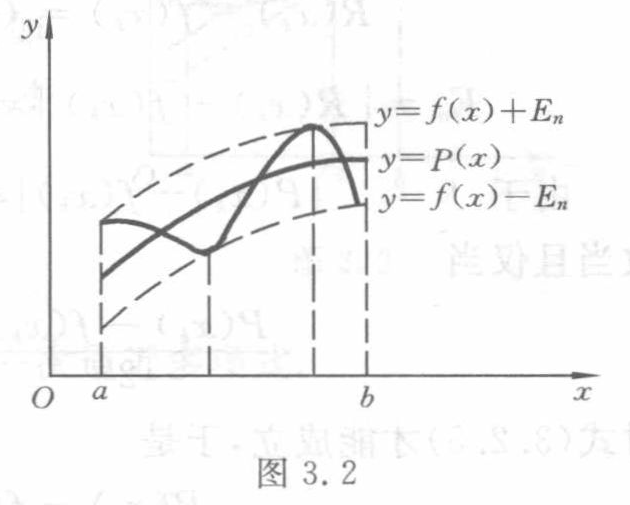
\includegraphics[width=0.85\linewidth,height=\textheight,keepaspectratio,alt={图 3.2 原图裁切}]{verified/assets/ch03a/fig-3-2.png}

图 3.2（原图）。带状区域及逼近曲线示意；标签为 \(x\)、\(y\)、\(O\)、\(a\)、\(b\)、\(y=f(x)+E_n\)、\(y=P(x)\)、\(y=f(x)-E_n\)。图内还画有从曲线接触点向横轴延伸的竖向辅助线。

定理 3.4 \(P(x) \in H_n\) 是 \(f(x) \in C[a,b]\) 的最佳逼近多项式的充分必要条件是 \(P(x)\) 在 \([a,b]\) 上至少有 \(n+2\) 个轮流为``正''、``负''的偏差点，即有 \(n+2\) 个点 \(a \leqslant x_1 < x_2 < \cdots < x_{n+2} \leqslant b\)，使

\[
\begin{aligned}
P(x_k)-f(x_k)&=(-1)^k\sigma\|P(x)-f(x)\|_\infty,\\
\sigma&=\pm1,\quad k=1,2,\cdots,n+2,
\end{aligned}
\tag{3.2.4}
\]

这样的点组称为 Chebyshev 交错点组.

证明 只证充分性. 假定在 \([a,b]\) 上有 \(n+2\) 个点使式 (3.2.4) 成立，要证明 \(P(x)\) 是 \(f(x)\) 在 \([a,b]\) 上的最佳逼近多项式. 用反证法求证. 若存在 \(Q(x) \in H_n, Q(x) \not\equiv P(x)\)，使

\[
\| f(x) - Q(x) \|_\infty < \| f(x) - P(x) \|_\infty.
\]

由于 \(P(x) - Q(x) = [P(x) - f(x)] - [Q(x) - f(x)]\) 在点 \(x_1, x_2, \cdots, x_{n+2}\) 上的符号与 \(P(x_k) - f(x_k)\) (\(k=1, \cdots, n+2\)) 一致，故 \(P(x) -\)

\begin{quote}
校注（agent 补充，原书疑误）：图 3.2 旁正文印为``定理 3.1 表明''，按原文保留。此段是在解释正、负偏差点同时存在，应指本页定理 3.3；定理 3.1 是 Weierstrass 定理。
\end{quote}

\clearpage

原书 PDF 页 63；印刷页码 50。

\href{source-images/pdf-063.jpeg}{查看原页}

\(Q(x)\) 也在 \(n+2\) 个点上轮流取符号``+''、``-''. 由连续函数性质, 它在 \((a,b)\) 内有 \(n+1\) 个零点, 但 \(P(x)-Q(x) \not\equiv 0\) 是不超过 \(n\) 次的多项式, 它的零点不超过 \(n\). 这个矛盾说明假设不对, 故 \(P(x)\) 就是所求最佳逼近多项式. 充分性得证.

必要性证明较繁, 但证明思想类似定理 3.3, 此处从略.

定理 3.4 说明, 用 \(P(x)\) 逼近 \(f(x)\) 的误差曲线 \(y=P(x)-f(x)\) 是均匀分布的. 由定理 3.4 还可得出以下重要推论.

推论 1 若 \(f(x) \in C[a,b]\), 则在 \(H_n\) 中存在唯一的最佳逼近多项式.

证明 若 \(H_n\) 中有两个最佳逼近多项式 \(P(x)\) 与 \(Q(x)\), 则对于一切 \(x \in [a,b]\), 都有 \[
-E_n \leqslant P(x)-f(x) \leqslant E_n, \quad -E_n \leqslant Q(x)-f(x) \leqslant E_n,
\] 于是 \[
-E_n \leqslant \frac{P(x)+Q(x)}{2}-f(x) \leqslant E_n.
\] 它表明 \(R(x)=\frac{Q(x)+P(x)}{2}\) 也是 \(H_n\) 中的最佳逼近多项式, 因而 \(R(x)-f(x)\) 的 \(n+2\) 个点的交错点组 \(\{x_k\}\) 满足 \[
R(x_k)-f(x_k)=(-1)^k \sigma E_n \quad (k=1,2,\cdots,n+2),
\] \[
E_n=\left|R(x_k)-f(x_k)\right|=\left|\frac{P(x_k)-f(x_k)}{2}+\frac{Q(x_k)-f(x_k)}{2}\right|. \tag{3.2.5}
\] 由于 \(\left|P(x_k)-f(x_k)\right| \leqslant E_n, \quad \left|Q(x_k)-f(x_k)\right| \leqslant E_n\), 故当且仅当 \[
\frac{P(x_k)-f(x_k)}{2}=\frac{Q(x_k)-f(x_k)}{2}=\pm \frac{E_n}{2}
\]

时式 (3.2.5) 才能成立, 于是 \[
P(x_k)-f(x_k)=Q(x_k)-f(x_k).
\] 这就得到 \(P(x_k)=Q(x_k)\) (\(k=1,2,\cdots,n+2\)), 从而表明 \(P(x)-Q(x)\) 有 \(n+2\) 个根. 这个矛盾说明 \(Q(x) \equiv P(x)\), 推论 1 得证.

推论 2 若 \(f(x) \in C[a,b]\), 则其最佳逼近多项式 \(P_n^*(x) \in H_n\) 就是 \(f(x)\) 的一个 Lagrange 插值多项式.

证明 由定理 3.4 可知, \(P_n^*(x)-f(x)\) 在 \([a,b]\) 上要么恒为零, 要么有 \(n+2\) 个轮流取``正''、``负''的偏差点, 于是存在 \(n+1\) 个点 \(x_k \leqslant \overline{x_k} \leqslant x_{k+1}\) (\(k=1,2,\cdots,n+1\)), 使 \(P_n^*(\overline{x_k})-f(\overline{x_k})=0\). 以 \(\overline{x_k}\) 为插值节点的 Lagrange 插值多项式就是 \(P_n^*(x)\).

\subsubsection{3.2.3 最佳一次逼近多项式}\label{ch03a-ux6700ux4f73ux4e00ux6b21ux903cux8fd1ux591aux9879ux5f0f}

定理 3.4给出了最佳逼近多项式 \(P(x)\) 的特性, 但要求出 \(P(x)\) 却相当困难. 下面先讨论 \(n=1\) 的情形.

假定 \(f(x) \in C^2[a,b]\), 且 \(f''(x)\) 在 \((a,b)\) 内不变号, 要求最佳一次逼近多项式

\clearpage

原书 PDF 页 64；印刷页码 51。

\href{source-images/pdf-064.jpeg}{查看原页}

\(P_1(x) = a_0 + a_1x\). 根据定理3.4可知，至少有3个点 \(a \leqslant x_1 < x_2 < x_3 \leqslant b\)，使 \(P_1(x_k) - f(x_k) = (-1)^k \sigma \max_{a \leqslant x \leqslant b} |P_1(x) - f(x)|\) (\(\sigma = \pm 1, k = 1, 2, 3\)).

由于 \(f''(x)\) 在 \([a, b]\) 上不变号，故 \(f'(x)\) 单调，\(f'(x) - a_1\) 在 \((a, b)\) 内只有一个零点，记作 \(x_2\)，于是 \(P_1'(x_2) - f'(x_2) = a_1 - f'(x_2) = 0\)，即 \(f'(x_2) = a_1\).

另外两个偏差点必在区间端点，即 \(x_0 = a, x_1 = b\)，且满足 \[
P_1(a) - f(a) = P_1(b) - f(b) = -[P_1(x_2) - f(x_2)] .
\] 由此得到 \[
\begin{cases} a_0 + a_1a - f(a) = a_0 + a_1b - f(b), \\ a_0 + a_1a - f(a) = f(x_2) - (a_0 + a_1x_2). \end{cases} \tag{3.2.6}
\]

解出 \[
a_1 = \frac{f(b) - f(a)}{b - a} = f'(x_2), \tag{3.2.7}
\] 代入式(3.2.6)，得 \[
a_0 = \frac{f(a) + f(x_2)}{2} - \frac{f(b) - f(a)}{b - a} \frac{a + x_2}{2}. \tag{3.2.8}
\]

这就得到最佳一次逼近多项式 \(P_1(x)\)，其几何意义如图3.3所示。直线 \(y = P_1(x)\) 与弦 \(MN\) 平行，且通过 \(MQ\) 的中点 \(D\)，其方程为 \[
y = \frac{1}{2}[f(a) + f(x_2)] + a_1\left(x - \frac{a + x_2}{2}\right).
\]

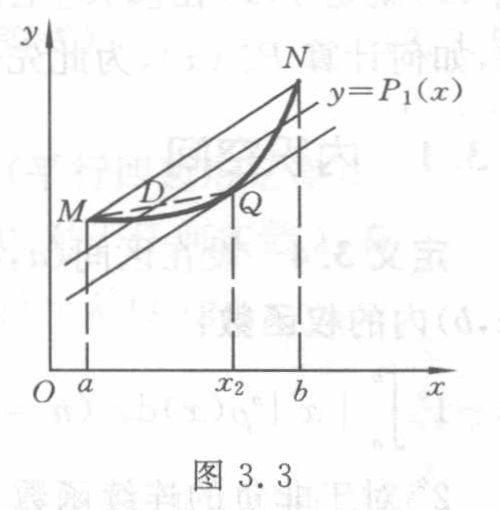
\includegraphics[width=0.85\linewidth,height=\textheight,keepaspectratio,alt={图 3.3 原图裁切}]{verified/assets/ch03a/fig-3-3.png}

图 3.3（原图）。最佳一次逼近的几何意义；标签为 \(x\)、\(y\)、\(O\)、\(a\)、\(x_2\)、\(b\)、\(M\)、\(N\)、\(Q\)、\(D\)、\(y=P_1(x)\)。弦 \(MN\)、逼近直线以及通过 \(Q\) 的平行线构成图中的三条斜线，\(D\) 为 \(MQ\) 的中点。

例3.1 求 \(f(x) = \sqrt{1+x^2}\) 在 \([0, 1]\) 上的最佳一次逼近多项式.

解 由式(3.2.7)可算出 \[
a_1 = \sqrt{2} - 1 \approx 0.414, \quad f'(x) = \frac{x}{\sqrt{1+x^2}},
\]

故 \[
\frac{x_2}{\sqrt{1+x_2^2}} = \sqrt{2} - 1,
\]

解得 \[
x_2 = \sqrt{\frac{\sqrt{2}-1}{2}} \approx 0.4551, \quad f(x_2) = \sqrt{1+x_2^2} \approx 1.0986.
\]

由式(3.2.8)，得 \[
a_0 = \frac{1 + \sqrt{1+x_2^2}}{2} - a_1 \frac{x_2}{2} \approx 0.955,
\]

于是得 \(\sqrt{1+x^2}\) 的最佳一次逼近多项式为 \[
P_1(x) = 0.955 + 0.414x,
\]

故 \[
\sqrt{1+x^2} \approx 0.955 + 0.414x, \quad 0 \leqslant x \leqslant 1. \tag{3.2.9}
\]

误差限为 \[
\max_{0 \leqslant x \leqslant 1} |\sqrt{1+x^2} - P_1(x)| \leqslant 0.045.
\]

\begin{quote}
校注（agent 补充，原书疑误）：本页开头先把三个交错点记为 \(x_1<x_2<x_3\)，随后原印``\(x_0=a,x_1=b\)''，此处忠实保留。按前文编号应为 \(x_1=a,x_3=b\)。
\end{quote}

\begin{quote}
校注（agent 补充，数值舍入）：原书对所写 \(P_1(x)=0.955+0.414x\) 给出误差限 \(0.045\)，这里保留原文。若把这两个已舍入系数当作精确数，则在 \(x=1\) 处误差为 \(\sqrt2-1.369\approx0.04521356>0.045\)，故所印误差限不适用于这组舍入后的系数。
\end{quote}

\clearpage

原书 PDF 页 65；印刷页码 52。

\href{source-images/pdf-065.jpeg}{查看原页}

在式(3.2.9)中若令 \(x = \frac{b}{a} \leqslant 1\), 则可得一个求根式的公式 \[
\sqrt{a^2 + b^2} \approx 0.955a + 0.414b.
\]

\subsection{3.3 最佳平方逼近}\label{ch03a-ux6700ux4f73ux5e73ux65b9ux903cux8fd1}

用均方误差最小作为度量标准, 研究函数 \(f(x) \in C[a,b]\) 的逼近多项式, 就是这一节要讨论的最佳平方逼近问题. 若存在 \(P_n^*(x) \in H_n\), 使 \[
\|f - P_n^*\|_2 = \sqrt{\int_a^b [f(x) - P_n^*(x)]^2 \mathrm{d}x} = \inf_{P \in H_n} \|f - P\|_2, \tag{3.3.1}
\] \(P_n^*(x)\) 就是 \(f(x)\) 在 \([a,b]\) 上的最佳平方逼近多项式. 这一节将研究 \(P_n^*(x)\) 是否存在, 如何计算 \(P_n^*(x)\), 为此先介绍一些有关内积空间的预备知识.

\subsubsection{3.3.1 内积空间}\label{ch03a-ux5185ux79efux7a7aux95f4}

定义3.4 设在区间 \((a,b)\) 内, 非负函数 \(\rho(x)\) 满足以下条件, 就称 \(\rho(x)\) 为区间 \((a,b)\) 内的权函数:

\(1^\circ \int_a^b |x|^n \rho(x) \mathrm{d}x (n = 0,1,\cdots)\) 存在;

\(2^\circ\) 对于非负的连续函数 \(g(x)\), 若 \[
\int_a^b g(x) \rho(x) \mathrm{d}x = 0, \tag{3.3.2}
\] 则在 \((a,b)\) 内 \(g(x) \equiv 0\).

定义3.5 设 \(f(x), g(x) \in C[a,b], \rho(x)\) 是 \([a,b]\) 上的权函数, 积分 \[
(f,g) = \int_a^b \rho(x) f(x) g(x) \mathrm{d}x \tag{3.3.3}
\] 称为函数 \(f(x)\) 与 \(g(x)\) 在 \([a,b]\) 上的内积.

容易验证这样定义的内积满足下列四条公理:

\begin{enumerate}
\def\labelenumi{(\arabic{enumi})}
\item
  \((f,g) = (g,f)\);
\item
  \((cf,g) = c(f,g), c\) 为常数;
\item
  \((f_1 + f_2, g) = (f_1, g) + (f_2, g)\);
\item
  \((f,f) \geqslant 0\), 当且仅当 \(f=0\) 时 \((f,f)=0\).
\end{enumerate}

满足内积定义的函数空间称为内积空间, 因此, 连续函数空间 \(C[a,b]\) 上定义了内积就形成一个内积空间. 这里定义的内积是 \(n\) 维 Euclid 空间 \(\mathbf{R}^n\) 中两个向量内积定义的推广, 设 \[
\boldsymbol{f} = (f_1, f_2, \cdots, f_n)^{\mathrm{T}}, \quad \boldsymbol{g} = (g_1, g_2, \cdots, g_n)^{\mathrm{T}},
\]

\clearpage

原书 PDF 页 66；印刷页码 53。

\href{source-images/pdf-066.jpeg}{查看原页}

其内积定义为 \((\boldsymbol{f}, \boldsymbol{g}) = \sum_{k=1}^{n} f_{k} g_{k}\); 向量 \(\boldsymbol{f} \in \mathbf{R}^{n}\) 的模(范数)定义为 \[
\| \boldsymbol{f} \|_{2} = \left( \sum_{k=1}^{n} f_{k}^{2} \right)^{\frac{1}{2}},
\] 将它推广到任何内积空间中就有下面的定义.

定义 3.6 \(f(x) \in C[a, b]\), 量 \[
\| f \|_{2} = \sqrt{\int_{a}^{b} \rho(x) f^{2}(x) \mathrm{d}x} = \sqrt{(f, f)} \tag{3.3.4}
\]

称为 \(f(x)\) 的 Euclid 范数.

它同样满足范数三条性质(见 3.1 节), 头两条是显然的, 下面定理包含了第三条性质和其他重要结论.

定理 3.5 对于任何 \(f, g \in C[a, b]\), 下列结论成立: \(1^{\circ}\)

\[
|(f,g)|\leqslant\|f\|_2\|g\|_2\qquad\text{(Cauchy-Schwarz 不等式)};\tag{3.3.5}
\] \(2^{\circ}\)

\[
\|f+g\|_2\leqslant\|f\|_2+\|g\|_2\qquad\text{(三角不等式)};\tag{3.3.6}
\] \(3^{\circ} \| f + g \|_{2}^{2} + \| f - g \|_{2}^{2} = 2(\| f \|_{2}^{2} + \| g \|_{2}^{2})\) (平行四边形定律).

证明 若 \(g=0\), 则式(3.3.5)显然成立, 现考虑 \(g \neq 0\). 对于任何实数 \(\lambda\), 有 \[
0 \leqslant (f + \lambda g, f + \lambda g) = (f, f) + 2\lambda(f, g) + \lambda^{2}(g, g).
\]

现取 \(\lambda = -\frac{(f, g)}{\| g \|_{2}^{2}}\), 代入上式得 \[
\| f \|_{2}^{2} - 2 \frac{|(f, g)|^{2}}{\| g \|_{2}^{2}} + \frac{|(f, g)|^{2}}{\| g \|_{2}^{2}} \geqslant 0, \quad |(f, g)|^{2} \leqslant \| f \|_{2}^{2} \| g \|_{2}^{2}.
\] 两边开平方即得式(3.3.5).

利用式(3.3.5)考虑 \[
\| f + g \|_{2}^{2} = (f + g, f + g) = (f, f) + 2(f, g) + (g, g)
\] \[
\leqslant \| f \|_{2}^{2} + 2 |(f, g)| + \| g \|_{2}^{2}
\] \[
\leqslant \| f \|_{2}^{2} + 2 \| f \|_{2} \| g \|_{2} + \| g \|_{2}^{2}
\] \[
= (\| f \|_{2} + \| g \|_{2})^{2},
\] 两边开方则得式(3.3.6).

平行四边形定律可直接计算得出, 可作为习题由读者完成. 证毕.

在 \(n\) 维空间中两个向量正交的定义也可推广到内积空间中.

定义 3.7 若 \(f(x), g(x) \in C[a, b]\) 满足 \[
(f, g) = \int_{a}^{b} \rho(x) f(x) g(x) \mathrm{d}x = 0, \tag{3.3.7}
\] 则称 \(f\) 与 \(g\) 在 \([a, b]\) 上带权 \(\rho(x)\) 正交. 若函数族 \(\varphi_{0}(x), \varphi_{1}(x), \cdots, \varphi_{n}(x), \cdots\) 满足关系 \[
(\varphi_{j}, \varphi_{k}) = \int_{a}^{b} \rho(x) \varphi_{j}(x) \varphi_{k}(x) \mathrm{d}x = \begin{cases} 0, & j \neq k, \\ A_{k} > 0, & j = k, \end{cases} \tag{3.3.8}
\]

\clearpage

原书 PDF 页 67；印刷页码 54。

\href{source-images/pdf-067.jpeg}{查看原页}

则称 \(\{\varphi_k\}\) 是 \([a,b]\) 上带权 \(\rho(x)\) 的正交函数族; 若 \(A_k \equiv 1\), 则称 \(\{\varphi_k\}\) 为标准正交函数族. 例如, 三角函数族 \[
1, \cos x, \sin x, \cos 2x, \sin 2x, \cdots
\] 就是在区间 \([-\pi, \pi]\) 上的正交函数族 (权 \(\rho(x) \equiv 1\)), 其 \[
(1,1) = 2\pi,
\] \[
(\sin nx, \sin mx) = \int_{-\pi}^{\pi} \sin nx \sin mx \mathrm{d}x = \begin{cases} \pi, & m=n, \\ 0, & m \neq n \end{cases} (n,m=1,2, \cdots),
\] \[
(\cos nx, \cos mx) = \int_{-\pi}^{\pi} \cos nx \cos mx \mathrm{d}x = \begin{cases} \pi, & m=n, \\ 0, & m \neq n \end{cases} (n,m=1,2, \cdots),
\] \[
(\cos nx, \sin mx) = \int_{-\pi}^{\pi} \cos nx \sin mx \mathrm{d}x = 0 (n,m=1,2, \cdots).
\] 在 \(\mathbf{R}^n\) 空间中, 任一向量都可用它的一组线性无关的基表示, 内积空间的任一元素 \(f(x) \in C[a,b]\) 也同样可用线性无关的基表示, 此时相应地有如下定义.

定义 3.8 设 \(\varphi_0(x), \varphi_1(x), \cdots, \varphi_{n-1}(x)\) 在 \([a,b]\) 上连续, 如果 \[
a_0 \varphi_0(x) + a_1 \varphi_1(x) + \cdots + a_{n-1} \varphi_{n-1}(x) = 0
\] 当且仅当 \(a_0 = a_1 = \cdots = a_{n-1} = 0\) 时成立, 则称 \(\varphi_0, \varphi_1, \cdots, \varphi_{n-1}\) 在 \([a,b]\) 上是线性无关的.

若函数族 \(\{\varphi_k\} (k=0,1, \cdots)\) 中的任何有限个 \(\varphi_k\) 线性无关, 则称 \(\{\varphi_k\}\) 为线性无关函数族.

例如, \(1, x, x^2, \cdots, x^n, \cdots\) 就是 \([a,b]\) 上的线性无关函数族. 若 \(\varphi_0(x), \varphi_1(x), \cdots, \varphi_{n-1}(x)\) 是 \([a,b]\) 上的线性无关函数, 且 \(a_0, a_1, \cdots, a_{n-1}\) 是任意实数, 则 \[
S(x) = a_0 \varphi_0(x) + a_1 \varphi_1(x) + \cdots + a_{n-1} \varphi_{n-1}(x)
\] 的全体是 \(C[a,b]\) 中的一个子集, 记作 \[
\Phi = \operatorname{span}\{\varphi_0, \varphi_1, \cdots, \varphi_{n-1}\}. \tag{3.3.9}
\] 下面给出判断函数族 \(\{\varphi_k\} (k=0,1, \cdots, n-1)\) 线性无关的充要条件.

定理 3.6 \(\varphi_0(x), \varphi_1(x), \cdots, \varphi_{n-1}(x)\) 在 \([a,b]\) 上线性无关的充分必要条件是它的 Cramer 行列式 \(G_{n-1} \neq 0\), 其中 \[
G_{n-1} = G(\varphi_0, \varphi_1, \cdots, \varphi_{n-1}) = \left| \begin{array}{cccc} (\varphi_0, \varphi_0) & (\varphi_0, \varphi_1) & \cdots & (\varphi_0, \varphi_{n-1}) \\ (\varphi_1, \varphi_0) & (\varphi_1, \varphi_1) & \cdots & (\varphi_1, \varphi_{n-1}) \\ \vdots & \vdots & & \vdots \\ (\varphi_{n-1}, \varphi_0) & (\varphi_{n-1}, \varphi_1) & \cdots & (\varphi_{n-1}, \varphi_{n-1}) \end{array} \right|. \tag{3.3.10}
\] 定理的证明由读者自行完成.

\subsubsection{3.3.2 函数的最佳平方逼近}\label{ch03a-ux51fdux6570ux7684ux6700ux4f73ux5e73ux65b9ux903cux8fd1}

下面研究在区间 \([a,b]\) 上一般的最佳平方逼近问题. 对 \(f(x) \in C[a,b]\) 及 \(C[a,b]\)

\begin{quote}
校注（agent 补充，原书术语疑误）：原页定理 3.6 写作``Cramer 行列式''，按原文保留。式 (3.3.10) 是由内积组成的 Gram 行列式，通常称``Gram（格拉姆）行列式''。
\end{quote}

\clearpage

原书 PDF 页 68；印刷页码 55。

\href{source-images/pdf-068.jpeg}{查看原页}

中的一个子集 \(\Phi = \text{span}\{\varphi_0, \varphi_1, \dots, \varphi_n\}\), 若存在 \(S^*(x) \in \Phi\), 使 \[
\| f - S^* \|_2^2 = \inf_{S \in \varphi} \| f - S \|_2^2 = \inf_{S \in \varphi} \int_a^b \rho(x) [f(x) - S(x)]^2 \mathrm{d}x, \tag{3.3.11}
\] 则称 \(S^*(x)\) 是 \(f(x)\) 在子集 \(\Phi \subseteq C[a, b]\) 中的最佳平方逼近函数. 为了求 \(S^*(x)\), 由式 (3.3.11)可知, 该问题等价于求多元函数 \[
I(a_0, a_1, \dots, a_n) = \int_a^b \rho(x) \left[ \sum_{j=0}^n a_j \varphi_j(x) - f(x) \right]^2 \mathrm{d}x \tag{3.3.12}
\] 的最小值. 由于 \(I(a_0, a_1, \dots, a_n)\) 是关于 \(a_0, a_1, \dots, a_n\) 的二次函数, 利用多元函数极值的必要条件 \[
\frac{\partial I}{\partial a_k} = 0 \quad (k = 0, 1, \dots, n),
\] \[
\frac{\partial I}{\partial a_k} = 2 \int_a^b \rho(x) \left[ \sum_{j=0}^n a_j \varphi_j(x) - f(x) \right] \varphi_k(x) \mathrm{d}x = 0 \quad (k = 0, 1, \dots, n),
\] 于是有 \[
\sum_{j=0}^n (\varphi_k, \varphi_j) a_j = (f, \varphi_k) \quad (k = 0, 1, \dots, n). \tag{3.3.13}
\] 这是关于 \(a_0, a_1, \dots, a_n\) 的线性方程组, 称为法方程. 由于 \(\varphi_0, \varphi_1, \dots, \varphi_n\) 线性无关, 故系数行列式 \(G(\varphi_0, \varphi_1, \dots, \varphi_n) \neq 0\), 于是方程组 (3.3.13) 有唯一解 \(a_k = a_k^* (k = 0, 1, \dots, n)\), 从而得到 \[
S^*(x) = a_0^* \varphi_0(x) + \dots + a_n^* \varphi_n(x).
\] 下面证明 \(S^*(x)\) 满足式 (3.3.11), 即对任何 \(S(x) \in \Phi\), 有 \[
\int_a^b \rho(x) [f(x) - S^*(x)]^2 \mathrm{d}x \leqslant \int_a^b \rho(x) [f(x) - S(x)]^2 \mathrm{d}x. \tag{3.3.14}
\] 为此只要考虑 \[
D = \int_a^b \rho(x) [f(x) - S(x)]^2 \mathrm{d}x - \int_a^b \rho(x) [f(x) - S^*(x)]^2 \mathrm{d}x
\] \[
= \int_a^b \rho(x) [S(x) - S^*(x)]^2 \mathrm{d}x + 2 \int_a^b \rho(x) [S^*(x) - S(x)] [f(x) - S^*(x)] \mathrm{d}x.
\] 由于 \(S^*(x)\) 的系数 \(a_k^*\) 是方程 (3.3.13) 的解, 故 \[
\int_a^b \rho(x) [f(x) - S^*(x)] \varphi_k(x) \mathrm{d}x = 0 \quad (k = 0, 1, \dots, n),
\] 从而上式第二个积分为零, 于是 \[
D = \int_a^b \rho(x) [S(x) - S^*(x)]^2 \mathrm{d}x \geqslant 0,
\] 故式 (3.3.14) 成立. 这就证明了 \(S^*(x)\) 是 \(f(x)\) 在 \(\Phi\) 中的最佳平方逼近函数. 若令 \(\delta = f(x) - S^*(x)\), 则平方误差为 \[
\|\delta\|_2^2 = (f - S^*, f - S^*) = (f, f) - (S^*, f) = \|f\|_2^2 - \sum_{k=0}^n a_k^* (\varphi_k, f). \tag{3.3.15}
\]

\begin{quote}
校注（agent 补充，原书符号不一致）：式 (3.3.11) 两处下确界下标原印 \(S\in\varphi\)（小写），本页前文子集定义为 \(\Phi\)（大写）。此处按原图保留小写，所指应为前文的 \(\Phi\)。
\end{quote}

\clearpage

原书 PDF 页 69；印刷页码 56。

\href{source-images/pdf-069.jpeg}{查看原页}

取 \(\varphi_k(x) = x^k, \rho(x) \equiv 1, f(x) \in C[0,1]\), 即要在 \(H_n\) 中求 \(n\) 次最佳平方逼近多项式

\[
S^*(x) = a_0^* + a_1^* x + \cdots + a_n^* x^n,
\]

此时

\[
(\varphi_j, \varphi_k) = \int_0^1 x^{k+j} \mathrm{d}x = \frac{1}{k+j+1},
\]

\[
(f, \varphi_k) = \int_0^1 f(x) x^k \mathrm{d}x \equiv d_k.
\]

若用 \(\boldsymbol{H}\) 表示行列式 \(G_n = G(1, x, x^2, \cdots, x^n)\) 对应的矩阵，则

\[\boldsymbol{H} = \begin{pmatrix}
1 & 1/2 & \cdots & 1/(n+1) \\
1/2 & 1/3 & \cdots & 1/(n+2) \\
\vdots & \vdots & & \vdots \\
1/(n+1) & 1/(n+2) & \cdots & 1/(2n+1)
\end{pmatrix}, \tag{3.3.16}
\]

\(\boldsymbol{H}\) 称为 Hilbert 矩阵. 记

\[
\boldsymbol{a} = (a_0, a_1, \cdots, a_n)^{\mathrm{T}}, \quad \boldsymbol{d} = (d_0, d_1, \cdots, d_n)^{\mathrm{T}},
\]

其中

\[
d_k = (f, x^k) (k=0, 1, \cdots, n), \tag{3.3.17}
\]

则方程

\[\boldsymbol{H}\boldsymbol{a}=\boldsymbol{d}
\]

的解 \(a_k = a_k^*\) (\(k=0, 1, \cdots, n\)) 即为所求.

例 3.2 设 \(f(x) = \sqrt{1+x^2}\), 求 \([0,1]\) 上的一次最佳平方逼近多项式.

解 利用式 (3.3.17), 得

\[
d_0 = \int_0^1 \sqrt{1+x^2} \mathrm{d}x = \frac{1}{2} \ln(1+\sqrt{2}) + \frac{\sqrt{2}}{2} \approx 1.147,
\]

\[
d_1 = \int_0^1 x \sqrt{1+x^2} \mathrm{d}x = \frac{1}{3} (1+x^2)^{\frac{3}{2}} \Bigg|_0^1 = \frac{2\sqrt{2}-1}{3} \approx 0.609,
\]

由方程组

\[
\begin{bmatrix}
1 & \frac{1}{2} \\
\frac{1}{2} & \frac{1}{3}
\end{bmatrix} \begin{pmatrix} a_0 \\ a_1 \end{pmatrix} = \begin{pmatrix} 1.147 \\ 0.609 \end{pmatrix},
\]

解出

\[
a_0 = 0.934, \quad a_1 = 0.426, \quad S_1^*(x) = 0.934 + 0.426x.
\]

平方误差

\[
\|\delta\|_2^2 = (f, f) - (S_1^*, f)
\]

\[
= \int_0^1 (1+x^2) \mathrm{d}x - 0.426 d_1 - 0.934 d_0 = 0.0026,
\]

最大误差

\[
\|\delta\|_\infty = \max_{0 \leqslant x \leqslant 1} |\sqrt{1+x^2} - S_1^*(x)| \approx 0.066.
\]

用 \(\{1, x, x^2, \cdots, x^n\}\) 作基求最佳平方逼近多项式, 当 \(n\) 较大时, 系数矩阵式 (3.3.16) 是高度病态的 (病态矩阵概念见第 7 章), 求法方程 (3.3.13) 的解时, 舍入误差很大, 这时, 用正交多项式作基才能求得最小平方逼近多项式 (见 3.5 节).

\begin{quote}
校注（agent 补充，数值舍入）：原书例 3.2 的系数与平方误差 \(0.0026\) 均按原文保留。该数值来自把 \(d_0,d_1\) 分别近似为 \(1.147,0.609\) 后代入简化式；对于印出的函数 \(S_1^*(x)=0.934+0.426x\)，直接计算 \(\int_0^1[\sqrt{1+x^2}-S_1^*(x)]^2\,\mathrm{d}x\approx0.0007136324\)，与 \(0.0026\) 不同。舍入后的系数不再严格满足精确内积对应的法方程，不能把简化式的数值视为实际平方误差。
\end{quote}

\clearpage

原书 PDF 页 70；印刷页码 57。

\href{source-images/pdf-070.jpeg}{查看原页}

\subsection{3.4 正交多项式}\label{ch03a-ux6b63ux4ea4ux591aux9879ux5f0f}

\subsubsection{3.4.1 正交化手续}\label{ch03a-ux6b63ux4ea4ux5316ux624bux7eed}

定义3.9 设 \(g_n(x)\) 是首项系数 \(a_n \neq 0\) 的 \(n\) 次多项式，如果多项式序列 \(g_0(x)\), \(g_1(x)\), \(\cdots\) 满足 \[
(g_j, g_k) = \int_a^b \rho(x) g_j(x) g_k(x) \mathrm{d}x = \begin{cases} 0, & j \neq k, \\ A_k > 0, & j = k \end{cases} \quad (j, k = 0, 1, \cdots),
\] 则称多项式序列 \(g_0(x), g_1(x), \cdots\) 在 \([a, b]\) 上带权 \(\rho(x)\) 正交，并称 \(g_n(x)\) 是 \([a, b]\) 上带权 \(\rho(x)\) 的 \(n\) 次正交多项式.

一般来说，当权函数 \(\rho(x)\) 及区间 \([a, b]\) 给定以后，可以由线性无关的一组基 \(\{1, x, x^2, \cdots, x^n, \cdots\}\) 并利用正交化方法构造出正交多项式 \[
g_0(x) = 1, \quad g_n(x) = x^n - \sum_{k=0}^{n-1} \frac{(x^n, g_k)}{(g_k, g_k)} \cdot g_k(x), \quad k = 1, 2, \cdots.
\] 这样构造的正交多项式有以下性质： (1) \(g_n(x)\) 是最高项系数为 1 的 \(n\) 次多项式. (2) 任一 \(n\) 次多项式 \(P_n(x) \in H_n\) 均可表示为 \(g_0(x), g_1(x), \cdots, g_n(x)\) 的线性组合. (3) 当 \(n \neq m\) 时，\((g_n, g_m) = 0\) 且 \(g_n(x)\) 与任一次数小于 \(n\) 的多项式正交. (4) 有递推关系 \[
g_{n+1}(x) = (x - \alpha_n)g_n(x) - \beta_n g_{n-1}(x), \quad n = 0, 1, \cdots,
\] 其中 \[
g_0(x) = 1, \quad g_{n-1}(x) = 0,
\] \[
\alpha_n = \frac{(xg_n, g_n)}{(g_n, g_n)}, \quad n = 0, 1, \cdots,
\] \[
\beta_n = \frac{(g_n, g_n)}{(g_{n-1}, g_{n-1})}, \quad n = 1, 2, \cdots.
\] 这里 \((xg_n, g_n) = \int_a^b xg_n^2(x) \rho(x) \mathrm{d}x.\) (5) 设 \(g_0(x), g_1(x), \cdots\) 是在 \([a, b]\) 上带权 \(\rho(x)\) 的正交多项式序列，则 \(g_n(x)\) (\(n \geq 1\)) 的 \(n\) 个根都是单重实根，且都在区间 \((a, b)\) 内. 以上性质的证明可参看相关文献. 下面主要给出几类常见的而又十分重要的正交多项式.

\subsubsection{3.4.2 Legendre多项式}\label{ch03a-legendreux591aux9879ux5f0f}

当区间为 \([-1, 1]\)、权函数 \(\rho(x) \equiv 1\) 时，由 \(\{1, x, x^2, \cdots, x^n, \cdots\}\) 正交化得到的多

\begin{quote}
校注（agent 补充，原书索引疑误）：本页正交化构造式末尾原印``\(k=1,2,\cdots\)''，而 \(k\) 已是求和哑指标，外部序号应为 \(n=1,2,\cdots\)；转录保留原式。
\end{quote}

\begin{quote}
校注（agent 补充，原书初值疑误）：递推初值原印 \(g_{n-1}(x)=0\)，按原文保留。若对一般 \(n\) 成立，会与 \(g_0(x)=1\) 冲突；递推通常应以 \(g_{-1}(x)=0\) 开始。
\end{quote}

\clearpage

原书 PDF 页 71；印刷页码 58。

\href{source-images/pdf-071.jpeg}{查看原页}

项式就称为 Legendre 多项式, 并用 \(P_0(x), P_1(x), \cdots, P_n(x), \cdots\) 表示. 这是 Legendre 于 1785 年引进的. 1814 年 Rodrigul 给出了简单的表达式

\[
P_0(x) = 1, \quad P_n(x) = \frac{1}{2^n n!} \frac{\mathrm{d}^n}{\mathrm{d}x^n} \{(x^2 - 1)^n\} \quad (n = 1, 2, \cdots). \tag{3.4.1}
\]

由于 \((x^2 - 1)^n\) 是 \(2n\) 次多项式, 求 \(n\) 阶导数后得

\[
P_n(x) = \frac{1}{2^2 n!} (2n)(2n - 1) \cdots (n + 1)x^n + a_{n-1}x^{n-1} + \cdots + a_0,
\]

于是得首项 \(x^n\) 的系数 \(a_n = \frac{(2n)!}{2^n (n!)^2}\). 显然最高项系数为 1 的 Legendre 多项式为

\[
\tilde{P}_n(x) = \frac{n!}{(2n)!} \frac{\mathrm{d}^n}{\mathrm{d}x^n} [(x^2 - 1)^n]. \tag{3.4.2}
\]

Legendre 多项式有以下几个重要性质.

性质 1 正交性

\[
\int_{-1}^{1} P_n(x) P_m(x) \mathrm{d}x = \begin{cases} 0, & m \neq n, \\ \frac{2}{2n + 1}, & m = n. \end{cases} \tag{3.4.3}
\]

证明 令 \(\varphi(x) = (x^2 - 1)^n\), 则

\[
\varphi^{(k)}(\pm 1) = 0 \quad (k = 0, 1, \cdots, n - 1).
\]

设 \(Q(x)\) 是区间 \([-1, 1]\) 上 \(n\) 阶连续可微的函数, 由分部积分知

\[
\int_{-1}^{1} P_n(x) Q(x) \mathrm{d}x = \frac{1}{2^n n!} \int_{-1}^{1} Q(x) \varphi^{(n)}(x) \mathrm{d}x = -\frac{1}{2^n n!} \int_{-1}^{1} Q'(x) \varphi^{(n-1)}(x) \mathrm{d}x
\]

\[
= \cdots = \frac{(-1)^n}{2^n n!} \int_{-1}^{1} Q^{(n)}(x) \varphi(x) \mathrm{d}x.
\]

下面分两种情况讨论.

\begin{enumerate}
\def\labelenumi{(\arabic{enumi})}
\tightlist
\item
  若 \(Q(x)\) 是次数小于 \(n\) 的多项式, 则 \(Q^{(n)}(x) \equiv 0\), 故当 \(m \neq n\) 时, 有
\end{enumerate}

\[
\int_{-1}^{1} P_m(x) P_n(x) \mathrm{d}x = 0.
\]

\begin{enumerate}
\def\labelenumi{(\arabic{enumi})}
\setcounter{enumi}{1}
\tightlist
\item
  若
\end{enumerate}

\[
Q(x) = P_n(x) = \frac{1}{2^n n!} \varphi^{(n)}(x) = \frac{(2n)!}{2^n (n!)^2} x^n + \cdots,
\]

\[
Q^{(n)}(x) = P_n^{(n)}(x) = \frac{(2n)!}{2^n n!},
\]

则

\[
\int_{-1}^{1} P_n^2(x) \mathrm{d}x = \frac{(-1)^n (2n)!}{2^{2n} (n!)^2} \int_{-1}^{1} (x^2 - 1)^n \mathrm{d}x = \frac{(2n)!}{2^{2n} (n!)^2} \int_{-1}^{1} (1 - x^2)^n \mathrm{d}x.
\]

由于

\[
\int_{0}^{1} (1 - x^2)^n \mathrm{d}x = \int_{0}^{\frac{\pi}{2}} \cos^{2n+1} t \mathrm{d}t = \frac{2 \cdot 4 \cdots 2n}{1 \cdot 3 \cdots (2n+1)},
\]

故当 \(m = n\) 时, 有

\[
\int_{-1}^{1} P_n^2(x) \mathrm{d}x = \frac{2}{2n+1}.
\]

证毕.

\begin{quote}
校注（agent 补充，原书系数疑误）：由 \((x^2-1)^n\) 求导后写出的 \(P_n(x)\) 首项系数中，原分母明确印为 \(2^2n!\)，此处按原文保留。依据式 (3.4.1)，该处应为 \(2^nn!\)；这也与紧随其后的 \(a_n=(2n)!/[2^n(n!)^2]\) 一致。
\end{quote}

\clearpage

原书 PDF 页 72；印刷页码 59。

\href{source-images/pdf-072.jpeg}{查看原页}

性质 2 奇偶性 \[
P_n(-x) = (-1)^n P_n(x). \tag{3.4.4}
\]

由于 \(\varphi(x) = (x^2 - 1)^n\) 是偶次多项式，经过偶次求导仍为偶次多项式，经过奇次求导则为奇次多项式，故 \(n\) 为偶数时 \(P_n(x)\) 为偶函数，\(n\) 为奇数时 \(P_n(x)\) 为奇函数，于是式(3.4.4)成立.

性质 3 递推关系 考虑 \(n+1\) 次多项式 \(xP_n(x)\)，它可表示为 \[
xP_n(x) = a_0P_0(x) + a_1P_1(x) + \cdots + a_{n+1}P_{n+1}(x),
\] 两边乘以 \(P_k(x)\)，并从 \(-1\) 到 \(1\) 积分，得 \[
\int_{-1}^{1} xP_n(x)P_k(x) \mathrm{d}x = a_k \int_{-1}^{1} P_k^2(x) \mathrm{d}x.
\] 当 \(k \leqslant n-2\) 时，\(xP_k(x)\) 次数不大于 \(n-1\)，上式左端积分为零，故得 \(a_k = 0\). 当 \(k=n\) 时 \(xP_n^2(x)\) 为奇函数，左端积分仍为零，故 \(a_n = 0\). 于是 \[
xP_n(x) = a_{n-1}P_{n-1}(x) + a_{n+1}P_{n+1}(x),
\] 其中 \[
a_{n-1} = \frac{2n-1}{2} \int_{-1}^{1} xP_n(x)P_{n-1}(x) \mathrm{d}x = \frac{2n-1}{2} \frac{2n}{4n^2-1} = \frac{n}{2n+1},
\] \[
a_{n+1} = \frac{2n+3}{2} \int_{-1}^{1} xP_n(x)P_{n+1}(x) \mathrm{d}x = \frac{2n+3}{2} \frac{2(n+1)}{(2n+1)(2n+3)} = \frac{n+1}{2n+1},
\] 从而得到以下的递推公式： \[
(n+1)P_{n+1}(x) = (2n+1)xP_n(x) - nP_{n-1}(x) \quad (n=1,2,\cdots). \tag{3.4.5}
\] 由 \(P_0(x)=1\)，\(P_1(x)=x\)， 利用式(3.4.5)就可推出 \[
P_2(x) = (3x^2 - 1)/2,
\] \[
P_3(x) = (5x^3 - 3x)/2,
\] \[
P_4(x) = (35x^4 - 30x^2 + 3)/8,
\] \[
P_5(x) = (63x^5 - 70x^3 + 15x)/8,
\] \[
P_6(x) = (231x^6 - 315x^4 + 105x^2 - 5)/16,
\] \[
\vdots
\] 图 3.4给出了 \(P_0(x), P_1(x), P_2(x), P_3(x)\) 的图形.

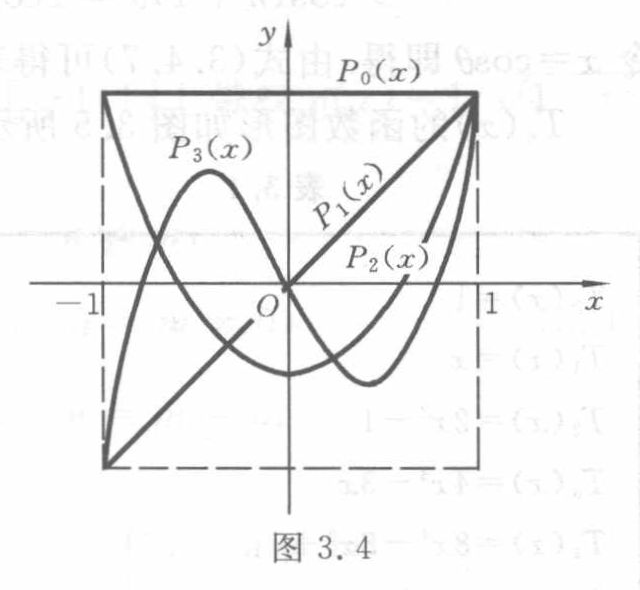
\includegraphics[width=0.85\linewidth,height=\textheight,keepaspectratio,alt={图 3.4 原图裁切}]{verified/assets/ch03a/fig-3-4.png}

图 3.4（原图）。Legendre 多项式 \(P_0(x)\)、\(P_1(x)\)、\(P_2(x)\)、\(P_3(x)\) 的图形。全部标签：\(x\)、\(y\)、\(O\)、\(-1\)、\(1\)、\(P_0(x)\)、\(P_1(x)\)、\(P_2(x)\)、\(P_3(x)\)；图中包含区间端点处的竖向及下边界虚线。

性质 4 在所有最高项系数为 1 的 \(n\) 次多项式中，Legendre 多项式 \(\widetilde{P}_n(x)\) 在 \([-1,1]\) 上与零的平方误差最小.

设 \(Q_n(x)\) 是任意一个最高项系数为 1 的 \(n\) 次多项式，它可表示为

\clearpage

原书 PDF 页 73；印刷页码 60。

\href{source-images/pdf-073.jpeg}{查看原页}

\[
Q_n(x) = \tilde{P}_n(x) + \sum_{k=0}^{n-1} a_k \tilde{P}_k(x) ,
\] 于是 \[
(Q_n, Q_n) = \int_{-1}^{1} Q_n^2(x) \mathrm{d}x = (\tilde{P}_n, \tilde{P}_n) + \sum_{k=0}^{n-1} a_k^2 (\tilde{P}_k, \tilde{P}_k) \geqslant (\tilde{P}_n, \tilde{P}_n)
\] 当且仅当 \(a_0 = a_1 = \cdots = a_{n-1} = 0\) 时等号才成立，即当 \(Q_n(x) \equiv \tilde{P}_n(x)\) 时平方误差最小.

性质 5 \(P_n(x)\) 在区间 \((-1, 1)\) 内有 \(n\) 个不同的实零点.

\subsubsection{3.4.3 Chebyshev多项式}\label{ch03a-chebyshevux591aux9879ux5f0f}

当权函数 \(\rho(x) = \frac{1}{\sqrt{1-x^2}}\), 区间为 \([-1, 1]\) 时, 由序列 \(\{1, x, x^2, \cdots, x^n, \cdots\}\) 正交化得到的正交多项式就是 Chebyshev多项式, 它可表示为 \[
T_n(x) = \cos(n \arccos x), \quad |x| \leqslant 1. \tag{3.4.6}
\] 若令 \(x = \cos \theta\), 则 \[
T_n(x) = \cos n \theta, \quad 0 \leqslant \theta \leqslant \pi.
\] Chebyshev多项式有很多重要性质.

性质 1 递推关系 \[
T_0(x) = 1, \quad T_1(x) = x,
\] \[
T_{n+1}(x) = 2xT_n(x) - T_{n-1}(x) \quad (n = 1, 2, \cdots). \tag{3.4.7}
\] 这只要由三角恒等式 \[
\cos(n+1)\theta = 2\cos \theta \cos n \theta - \cos(n-1)\theta \quad (n \geqslant 1)
\] 令 \(x = \cos \theta\) 即得. 由式(3.4.7)可得表 3.1.

\(T_n(x)\) 的函数图形如图 3.5 所示.

表 3.1

{\def\LTcaptype{none} % do not increment counter
\begin{longtable}[]{@{}ll@{}}
\toprule\noalign{}
多项式 & 表达式 \\
\midrule\noalign{}
\endhead
\bottomrule\noalign{}
\endlastfoot
\(T_0(x)\) & \(1\) \\
\(T_1(x)\) & \(x\) \\
\(T_2(x)\) & \(2x^2-1\) \\
\(T_3(x)\) & \(4x^3-3x\) \\
\(T_4(x)\) & \(8x^4-8x^2+1\) \\
\(T_5(x)\) & \(16x^5-20x^3+5x\) \\
\(T_6(x)\) & \(32x^6-48x^4+18x^2-1\) \\
\(T_7(x)\) & \(64x^7-112x^5+56x^3-7x\) \\
\(T_8(x)\) & \(128x^8-256x^6+160x^4-32x^2+1\) \\
\end{longtable}
}

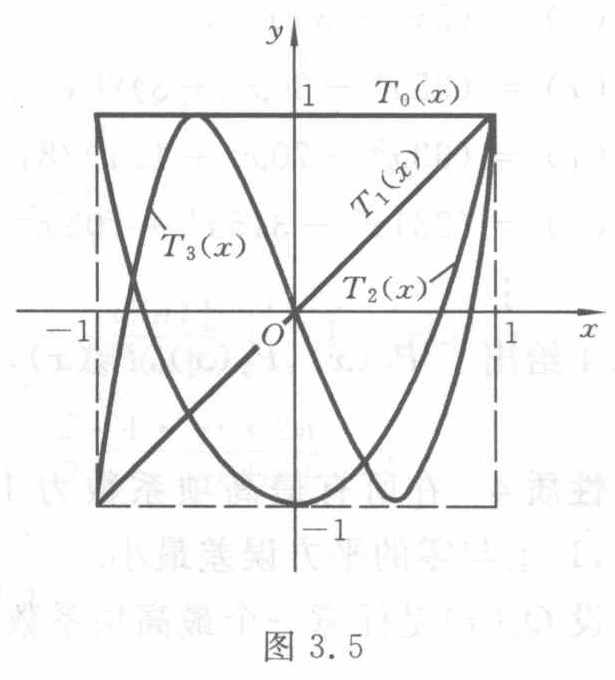
\includegraphics[width=0.85\linewidth,height=\textheight,keepaspectratio,alt={图 3.5 原图裁切}]{verified/assets/ch03a/fig-3-5.png}

图 3.5（原图）。Chebyshev 多项式 \(T_0(x)\)、\(T_1(x)\)、\(T_2(x)\)、\(T_3(x)\) 的图形。全部标签：\(x\)、\(y\)、\(O\)、横轴的 \(-1\)、\(1\)、纵轴的 \(1\)、\(-1\)、\(T_0(x)\)、\(T_1(x)\)、\(T_2(x)\)、\(T_3(x)\)；在 \(x=\pm1\) 处画有辅助线。

\clearpage

原书 PDF 页 74；印刷页码 61。

\href{source-images/pdf-074.jpeg}{查看原页}

由递推关系式(3.4.7)还可得到 \(T_n(x)\) 的最高项系数是 \(2^{n-1}(n \geqslant 1)\).

性质 2 \(T_n(x)\) 对零的偏差最小. 它可写成如下定理.

定理 3.7 在区间 \([-1,1]\) 上所有最高项系数为 1 的一切 \(n\) 次多项式中, \(\omega_n(x) = \frac{1}{2^{n-1}} T_n(x)\) 与零的偏差最小, 其偏差为 \(\frac{1}{2^{n-1}}\).

证明 由于 \(\omega_n(x) = \frac{1}{2^{n-1}} T_n(x) = x^n - P_{n-1}^*(x)\),

\[
\max_{-1 \leqslant x \leqslant 1} |\omega_n(x)| = \frac{1}{2^{n-1}} \max_{-1 \leqslant x \leqslant 1} |T_n(x)| = \frac{1}{2^{n-1}} ,
\] 且点 \(x_k = \cos \frac{k}{n}\pi (k=0,1,\cdots,n)\) 是 \(T_n(x)\) 的 Chebyshev 交错点组, 由定理 3.4 可知, 在区间 \([-1,1]\) 上, \(x^n\) 在 \(H_{n-1}\) 中最佳逼近多项式为 \(P_{n-1}^*(x)\), 即 \(\omega_n(x)\) 是与零的偏差最小的多项式. 证毕.

例 3.3 求 \(f(x) = 2x^3 + x^2 + 2x - 1\) 在 \([-1,1]\) 上的最佳二次逼近多项式.

解 由题意, 所求最佳逼近多项式 \(P_{2}^*(x)\) 应满足

\[
\max_{-1 \leqslant x \leqslant 1} |f(x) - P_{2}^*(x)| = \min .
\] 由定理 3.6 可知, 当

\[
f(x) - P_{2}^*(x) = \frac{1}{2} T_3(x) = 2x^3 - \frac{3}{2}x
\] 时, 与零偏差最小, 故

\[
P_{2}^*(x) = f(x) - \frac{1}{2} T_3(x) = x^2 + \frac{7}{2}x - 1
\] 就是 \(f(x)\) 在 \([-1,1]\) 上的最佳二次逼近多项式.

性质 3 Chebyshev 多项式 \(\{T_k(x)\}\) 在区间 \([-1,1]\) 上带权 \(\rho(x) = 1 / \sqrt{1-x^2}\) 正交, 且

\[
\int_{-1}^{1} \frac{T_n(x)T_m(x)\,\mathrm{d}x}{\sqrt{1-x^2}} = \begin{cases} 0, & n \neq m, \\ \frac{\pi}{2}, & n = m \neq 0, \\ \pi, & n = m = 0. \end{cases} \tag{3.4.8}
\]

事实上, 令 \(x = \cos \theta\), 则 \(\mathrm{d}x = -\sin \theta \mathrm{d}\theta\), 于是

\[
\int_{-1}^{1} \frac{T_n(x)T_m(x)}{\sqrt{1-x^2}} \mathrm{d}x = \int_{0}^{\pi} \cos n\theta \cos m\theta \mathrm{d}\theta = \begin{cases} 0, & n \neq m, \\ \frac{\pi}{2}, & n = m \neq 0, \\ \pi, & n = m = 0. \end{cases}
\]

性质 4 \(T_{2k}(x)\) 只含 \(x\) 的偶次幂, \(T_{2k+1}(x)\) 只含 \(x\) 的奇次幂.

此性质由递推关系直接得到.

\begin{quote}
校注（agent 补充，原书交叉引用疑误）：例 3.3 中原文写``由定理 3.6 可知''，照录。此处使用的是本页定理 3.7 的最小偏差性质；定理 3.6 是线性无关与内积行列式的判别条件。
\end{quote}

\clearpage

原书 PDF 页 75；印刷页码 62。

\href{source-images/pdf-075.jpeg}{查看原页}

性质 5 \(T_n(x)\) 在区间 \([-1,1]\) 上有 \(n\) 个零点 \(x_k = \cos \frac{2k-1}{2n}\pi, k=1, \cdots, n\). 此外, 实际计算中时常要求 \(x^n\) 用 \(T_0, T_1, \cdots, T_n\) 的线性组合表示, 其公式为 \[
x^n = 2^{1-n} \sum_{k=0}^{[\frac{n}{2}]} \binom{n}{k} T_{n-2k}(x). \tag{3.4.9}
\]

这里规定 \(T_0 = 1/2\). \(n=1 \sim 8\) 的结果如表 3.2 所示.

表 3.2

{\def\LTcaptype{none} % do not increment counter
\begin{longtable}[]{@{}ll@{}}
\toprule\noalign{}
幂函数 & Chebyshev 多项式表示 \\
\midrule\noalign{}
\endhead
\bottomrule\noalign{}
\endlastfoot
\(1\) & \(T_0\) \\
\(x\) & \(T_1\) \\
\(x^2\) & \(\frac12(T_0+T_2)\) \\
\(x^3\) & \(\frac14(3T_1+T_3)\) \\
\(x^4\) & \(\frac18(3T_0+4T_2+T_4)\) \\
\(x^5\) & \(\frac1{16}(10T_1+5T_3+T_5)\) \\
\(x^6\) & \(\frac1{32}(10T_0+15T_2+6T_4+T_6)\) \\
\(x^7\) & \(\frac1{64}(35T_1+21T_3+7T_5+T_7)\) \\
\(x^8\) & \(\frac1{128}(35T_0+56T_2+28T_4+8T_6+T_8)\) \\
\end{longtable}
}

\subsubsection{3.4.4 其他常用的正交多项式}\label{ch03a-ux5176ux4ed6ux5e38ux7528ux7684ux6b63ux4ea4ux591aux9879ux5f0f}

一般地说, 如果区间 \([a,b]\) 及权函数 \(\rho(x)\) 不同, 则得到的正交多项式也不同. 除上述两种最重要的正交多项式外, 下面再给出三种较常用的正交多项式.

\paragraph{1. 第二类 Chebyshev 多项式}\label{ch03a-ux7b2cux4e8cux7c7b-chebyshev-ux591aux9879ux5f0f}

在区间 \([-1,1]\) 上带权 \(\rho(x) = \sqrt{1-x^2}\) 的正交多项式称为第二类 Chebyshev 多项式, 其表达式为

\[
U_n(x) = \frac{\sin[(n+1)\arccos x]}{\sqrt{1-x^2}}. \tag{3.4.10}
\]

由 \(x=\cos\theta\) 可得

\[
\int_{-1}^{1} U_n(x) U_m(x) \sqrt{1-x^2} \mathrm{d}x = \int_{0}^{\pi} \sin(n+1)\theta \sin(m+1)\theta \mathrm{d}\theta
\]

\[
= \left\{ \begin{array}{l l} 0, & m \neq n, \\ \frac{\pi}{2}, & m=n, \end{array} \right.
\]

\begin{quote}
校注（agent 补充，记号约定）：式 (3.4.9) 后原文规定 \(T_0=1/2\)，而表 3.2 首行原印 \(1=T_0\)；两处均忠实保留。式 (3.4.9) 的求和使用临时的半权常数项约定，表 3.2 则与前文通常定义 \(T_0=1\) 一致。使用时须区分这两种约定。
\end{quote}

